%--------------------
% Packages
% -------------------
\documentclass[11pt,a4paper]{article}
\usepackage[utf8x]{inputenc}
\usepackage[T1]{fontenc}
\usepackage{mathptmx}


\usepackage[pdftex]{graphicx}
\usepackage[pdftex,linkcolor=black,pdfborder={0 0 0}]{hyperref}
\usepackage{calc}
\usepackage{enumitem}

\frenchspacing 
\linespread{1.2}
\usepackage[a4paper, lmargin=0.1666\paperwidth, rmargin=0.1666\paperwidth, tmargin=0.1111\paperheight, bmargin=0.1111\paperheight]{geometry} %margins

\usepackage[all]{nowidow}
\usepackage[protrusion=true,expansion=true]{microtype}


%-----------------------
% Set pdf information and add title, fill in the fields
%-----------------------
\hypersetup{ 	
pdfsubject = {},
pdftitle = {},
pdfauthor = {}
}

%-----------------------
% Begin document
%-----------------------
\begin{document}

\title{Software Testing - A3}
\author{Ingmar Falk}
\maketitle
\pagebreak

\section{Introduction}

In this report, I will analyze the paper \textit{To Mock or Not To Mock? - An Empirical Study on Mocking Practices}, by the \textit{Delft University of Technology}.
To collect data for this paper, the researchers conducted a survey among developers from a handful of projects as well as created a 
tool to collect statistics about the usage of mocking in the tests of said projects. Among those projects are \textit{SonarQube},
the \textit{Spring Framework}, \textit{VRaptor} and \textit{Alura}. All of these projects are written in Java and use javas most popular
mocking framework \textit{Mockito}.

\section{Methodology}

\subsection{Data Collection}

The goal of this paper was to investigate how and why developers make use of mock objects when writing tests. There are 3 main
questions, that were applied to all projects:

\begin{itemize}
    \item What test dependencies do developers mock?
    \item Why do developers decide to (not) mock specific dependencies?
    \item What are the main challenges experienced with testing using mocks?
\end{itemize}

To answer these questions the team created a tool called \emph{\textit{MockExtracor}}. Using this tool, they extracted data
about all of the classes, lines of code, tests with/without mocks and other information useful for later analysis.

\begin{figure}[h]
    \centering
    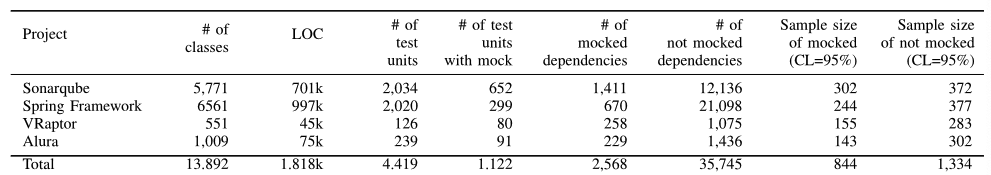
\includegraphics[width=0.8\textwidth]{images/source.png}
    \caption{Image taken from the paper, showing the data collected from the projects}
\end{figure}

\subsection{Analysis}

Due to the size of the projects and the amount of data collected, the team decided to only use a random sample of the original data.
Defining an automated analysis process would have been extremely challenging, so the researchers went with a manual approach.
Each of the researchers was responsible for two projects, which they then analyzed by hand and entered the data into a spreadsheet.
One of the main objectives of this analysis was to assign broad categories to each analyzed unit.

\subsection{Categorization}

After assigning a category to each unit in the analysis stage, it was now time to merge the categories to reduce the number
from 116 to a more manageable number. This was done by grouping similar categories together and then merging them into one.
In total, the researchers ended up with 7 categories, which are:
\textit{Database}
, \textit{Web Service}
, \textit{External Dependencies}
, \textit{Domain Object}
, \textit{Java Libraries}
, \textit{Test Support}.

\begin{figure}[h]
    \centering
    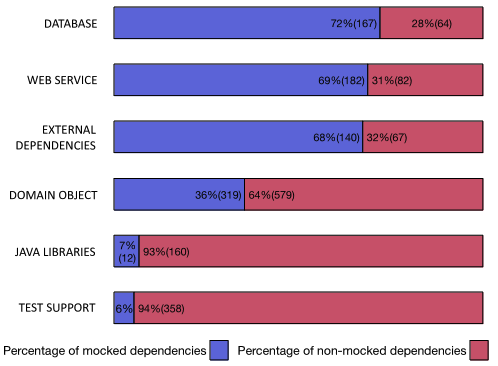
\includegraphics[width=0.8\textwidth]{images/categories.png}
    \caption{Image taken from the paper, showing the final categories}
\end{figure}

\subsection{Interviews}

To get a better understanding of the data, the researchers conducted interviews with developers from the projects and inquired
about their testing practices and the usage of mocks. The interviews were semi-structured, meaning that the researchers had
a set of questions prepared, but were also free to ask follow-up questions. The prepared questions were based on the data 
collected in the previous steps. The interviewers made sure to ask questions about the interviewee's reasoning for (not) mocking
a certain category of dependencies, exceptions and the pros and cons regarding that category.

\pagebreak

\subsection{Survey}

The survey was also based on all previous stages and aimed to expand upon the concepts that emerged from them. The questions were
all based on the previously discovered data. It consisted of 4 main parts:

\begin{itemize}
    \item Part 1. Participants experience in Software Development and Mocking
    \item Part 2. How often do participants make use of mocks in each found category
    \item Part 3. How often do participants make use of mocks in specific situations (complex, coupled, slow, etc.)
    \item Part 4. Challenges of mocking (Open-ended and Optional)
\end{itemize}

They received 105 responses. Experience:

\begin{itemize}
    \item 21 \% -- 1-5 years
    \item 64 \% -- 6-15 years
    \item 15 \% -- 16+ years
\end{itemize}

With the languages used:

\begin{itemize}
    \item 24 \% -- Java
    \item 18 \% -- C\#
    \item 19 \% -- JavaScript
    \item Other
\end{itemize}

\section{Threats to Validity}

\subsection{Construct Validity}

The study acknowledges potential issues with the research instruments, 
particularly the use of MOCKEXTRACTOR for collecting dependencies through static 
code analysis. This tool may not capture dynamic behaviors, leading to 
some dependencies being incorrectly categorized as "non-mocked." 
The study mitigates this by using random samples in manual analysis and 
manually inspecting MOCKEXTRACTOR results in 100 test units, 
which showed no issues in those cases. Agreement among researchers analyzing 
the data was 89\%.

\subsection{Internal Validity}

Concerns are raised about factors not considered that could affect the 
variables and relationships being investigated. The study interviews developers to 
understand why certain dependencies are mocked or not, but a single developer 
may not have complete knowledge of all implementation decisions. 
To address this, the study presents data from the first research question first and 
avoids asking questions about overall categories coined in RQ1. 
The potential influence of other factors, like current literature and other projects, 
is also acknowledged, and interviewees are reminded to focus on their specific project.

\subsection{External Validity}

There are concerns about the generalizability of the results due to a small sample size, 
consisting of four Java systems (one of them being closed source). 
To mitigate this, the opinions of 105 developers from various projects are collected. 
The study suggests that further research in different projects and programming languages 
should be conducted. Additionally, there may be self-selection bias in the 
survey respondents and the study lacks information about the nature of the 
the overall population that responded to the survey.

\section{Results}

\subsection{RQ1: What test dependencies do developers mock?}

The categories explained are as follows:

\begin{itemize}
    \item Domain object: Classes that contain system rules, often dependent on other domain objects and not external resources.
    \item Database: Classes interacting with external databases, either as external libraries or as classes depending on such libraries.
    \item Native Java libraries: Java's built-in libraries, such as Java I/O and Java Util classes.
    \item Web Service: Classes performing HTTP actions, similar to databases in terms of external dependencies.
    \item External dependency: Libraries or classes using external libraries outside the project.
    \item Test support: Classes that support testing, like fake domain objects, test data builders, and web services for testing.
    \item Unresolved: Dependencies that couldn't be resolved, often from sub-modules with unavailable source code.
\end{itemize}

The percentage of mocked dependencies varies across projects,
with databases and domain objects showing some differences. 
For instance, Sonarqube mocks around 47\% of domain object dependencies, while other projects mock them around 30\% of the time.
For databases, SonarQube and Alura mock around 60\% of the dependencies, while Spring mocks 94\% of them.
Web services and databases are the most frequently mocked dependencies,
while domain objects exhibit a less clear trend with around 36\% of them being mocked
Test support and Java libraries are almost never mocked, which is expected since the former includes classes specifically created to support testing, 
and the latter comprises Java's core libraries that are typically reliable and don't require mocking

\subsection{RQ2: Why do developers decide to (not) mock specific dependencies?}

\begin{itemize}
    \item Mocks are commonly used when the concrete implementation of a dependency is not simple. Dependencies that are highly coupled, complex to set up, contain complex code, perform slow tasks, or rely on external resources (e.g., databases, web services, or external libraries) are often candidates for mocking.
    \item Developers prefer not to use mocks when testing the integration with an external dependency itself, as they want to ensure that the integration works correctly. However, they do use mocks when unit testing a class that depends on a class dealing with external resources to isolate the unit being tested.
    \item Interfaces are often mocked instead of specific implementations to avoid relying on a particular implementation.
    \item Domain objects are usually not mocked, especially when they are simple and don't deal with external resources. However, complex domain objects or highly coupled ones may be mocked.
    \item Native Java objects and libraries, which are easy to instantiate with desired values, are typically not mocked. However, there may be exceptions, such as dealing with complex file operations.
    \item Database, web services, and external dependencies are considered good candidates for mocking due to their complexity and slow setup. Developers commonly mock these dependencies when testing.
    \item The decision to mock or not mock depends on whether the focus of testing is on the integration itself. When integration testing is required, mocks are less likely to be used, but for unit testing, mocks are preferred for certain types of dependencies.
    \item Survey respondents generally align with the interviewees' perspectives, indicating a preference for mocking web services, external dependencies, and databases when not testing integration
\end{itemize}

\subsection{RQ3: What are the main challenges experienced with testing using mocks?}

\begin{itemize}
    \item Dealing with Coupling: Mocking practices can introduce coupling between tests and production code. Additionally, high coupling among production classes can make mocking challenging, especially when proper decoupling and dependency isolation haven't been implemented.
    \item Getting Started with Mocks: Mocks may be a new concept for some developers, requiring experienced developers to teach junior developers. Some developers may struggle to understand and use mock objects effectively.
    \item Mocking in Legacy Systems: Testing single units in legacy systems may require extensive mocking, sometimes even mocking the entire system. Tools like PowerMock may be necessary for classes not designed for testability. In some cases, mocking is the only way to perform unit testing in legacy systems with poor architecture.
    \item Non-Testable/Hard-to-Test Classes: Various technical details can hinder the use of mock objects, such as static methods in Java, file uploads in PHP, interfaces in dynamic languages, and specific language features like LINQ in C\#.
    \item Relationship Between Mocks and Code Quality: Excessive use of mocks is seen as an indicator of poorly engineered code. Mocks can hide deeper problems in the system's design, such as highly coupled and complex classes. Well-structured production code should ideally require fewer mocks. Using too many mocks may lead to test readability and maintenance issues.
    \item Unstable Dependencies: Maintaining the behavior of mock objects compatible with the behavior of the original class can be challenging, especially when the production class frequently changes. Poorly designed or highly coupled production classes can make mock objects more unstable and prone to change.
\end{itemize}


\pagebreak

\end{document}
